% Figure s01f01_fockspace (Session 1): one hopping matrix against the Fock space of three sites.
% The image is rendered by figures/blender/s01f01_fockspace.py; the coordinates of the labels come from
% figures/blender/out/s01f01_fockspace_anchors.tex. Build with figures/blender/build_figure.sh s01f01_fockspace.
\documentclass[11pt,tikz,border=0pt]{standalone}
\usepackage[T1]{fontenc}
\usepackage{amsmath,amssymb,graphicx}
\usepackage{xcolor}
\usetikzlibrary{arrows.meta,calc}
% The three label colors of the figures, with the same values as in src/figures_preamble.tex.
\definecolor{aqmaccent}{RGB}{31,78,121}
\definecolor{aqmbroken}{RGB}{168,42,34}
\definecolor{aqmmuted}{RGB}{125,125,125}

\newlength{\figw}\setlength{\figw}{18.23cm}   % 1.17 of the text width, before the empty margins of the render are cropped

\begin{document}
\begin{tikzpicture}[lbl/.style={font=\small, inner sep=1.5pt},
    flow/.style={line width=0.9pt, -{Stealth[length=5pt,width=4pt]}}]
  \node[overlay, anchor=south west, inner sep=0pt] at (0,0)
    {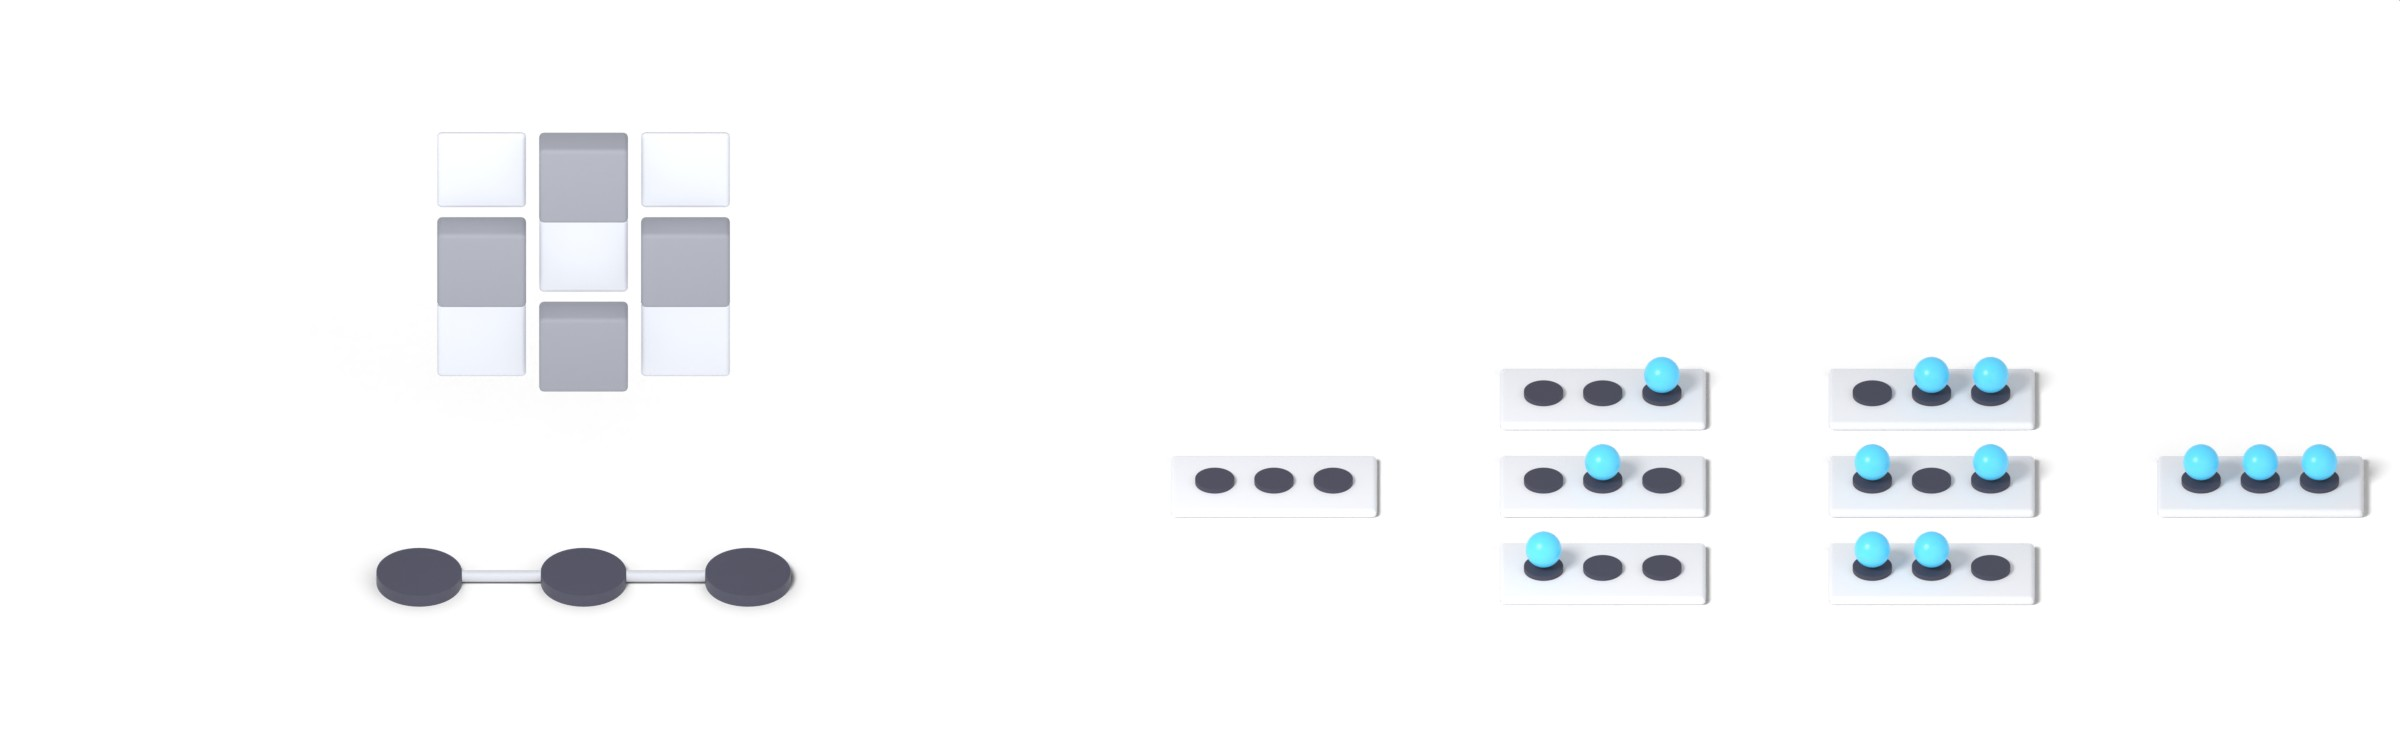
\includegraphics[width=\figw]{../blender/out/s01f01_fockspace.jpg}};
  % written by build_figure.sh; the painted part of the image
\path (0.1508\figw,0.0575\figw) rectangle (0.9946\figw,0.2575\figw);

  %% written by figlib.py; x and y in units of the image width
\coordinate (mat) at (0.3103\figw,0.2075\figw);
\coordinate (titleA) at (0.2432\figw,0.2688\figw);
\coordinate (chain) at (0.2432\figw,0.0524\figw);
\coordinate (N0) at (0.5308\figw,0.1635\figw);
\coordinate (c0) at (0.5308\figw,0.0524\figw);
\coordinate (N1) at (0.6678\figw,0.1635\figw);
\coordinate (c1) at (0.6678\figw,0.0524\figw);
\coordinate (N2) at (0.8048\figw,0.1635\figw);
\coordinate (c2) at (0.8048\figw,0.0524\figw);
\coordinate (N3) at (0.9418\figw,0.1635\figw);
\coordinate (c3) at (0.9418\figw,0.0524\figw);
\coordinate (titleB) at (0.7363\figw,0.2061\figw);

  \node[lbl, anchor=south] at (titleA) {first quantization};
  \node[lbl, anchor=west] at (mat) {$L\times L$};
  \node[lbl, anchor=north] at (chain) {$L=3$ sites};
  \node[lbl, anchor=south] at (titleB) {second quantization, the full Fock space};
  \node[lbl, anchor=south, text=aqmmuted] at (N0) {$N=0$};
  \node[lbl, anchor=south, text=aqmmuted] at (N1) {$N=1$};
  \node[lbl, anchor=south, text=aqmmuted] at (N2) {$N=2$};
  \node[lbl, anchor=south, text=aqmmuted] at (N3) {$N=3$};
  \node[lbl, anchor=north, text=aqmaccent] at (c0) {$1$};
  \node[lbl, anchor=north, text=aqmaccent] at (c1) {$3$};
  \node[lbl, anchor=north, text=aqmaccent] at (c2) {$3$};
  \node[lbl, anchor=north, text=aqmaccent] at (c3) {$1$};
  \node[lbl, anchor=north] at ($(c1)!0.5!(c2)+(0,-0.45cm)$) {$1+3+3+1=2^L=8$ states};
\end{tikzpicture}
\end{document}
